\section{Results}
\label{sec:result}

\subsection{Experimental Setup}

\textbf{Datasets.}
We build our study on a comprehensive collection of twelve representative low-level vision tasks. Specifically, we use GOPRO~\cite{nah2017deep} for image deblurring, D-HAZY~\cite{ancuti2016d} for dehazing, UHDM~\cite{yu2022towards} for demoireing, SIDD~\cite{abdelhamed2018high, abdelhamed2020ntire} for denoising, RainCityscapes~\cite{hu2019depth} for deraining, iHarmony4~\cite{cong2019image} for harmonization, DIV2K~\cite{agustsson2017ntire} with modifications for inpainting and colorization, LoL~\cite{wei2018deep} for low-light enhancement, SIR$^2$~\cite{wan2022benchmarking} for reflection removal, ISTD~\cite{wang2018stacked} for shadow removal, and Night2Day~\cite{laffont2014transient} for style transfer. Details are provided in Appendix Sec.~\ref{sec:data}. We perform experiments that scale quadratically with the number of task pairs.

\noindent \textbf{Implementation details.} We conducted our experiments using two NVIDIA A100-SXM4 GPUs with 80 GB of memory each. We follow each dataset's standard train-test split whenever available, or adopt a 70/30 random division when no official split is provided. All images are resized to a unified resolution ($448 \times 448$ for training inputs, $224 \times 224$ for query inputs) to maintain compatibility with the VLM framework.

\subsection{Cross-Task Results in Top-Tier Group}
Table~\ref{tab:3} presents quantitative comparisons across twelve representative task pairs on Gemini and Seedream, each compared with its fixed-prompt baseline.
Figure~\ref{fig:fig4} illustrates representative examples of cross-task ICL on Gemini, demonstrating how the VLM adapts flexibly to diverse tasks driven by conditioning implicit text prompts. Among these tasks, at least two of the three evaluation metrics consistently outperform the fixed-prompt baseline for both models, and the third metric remains very close. Notably, VIEScore improves throughout, highlighting the effectiveness of our implicit prompt-driven generalization mechanism. Additional relevant qualitative examples are provided in Appendix Sec.~\ref{sec:example}.

\begin{figure*}[ht]
    \centering
    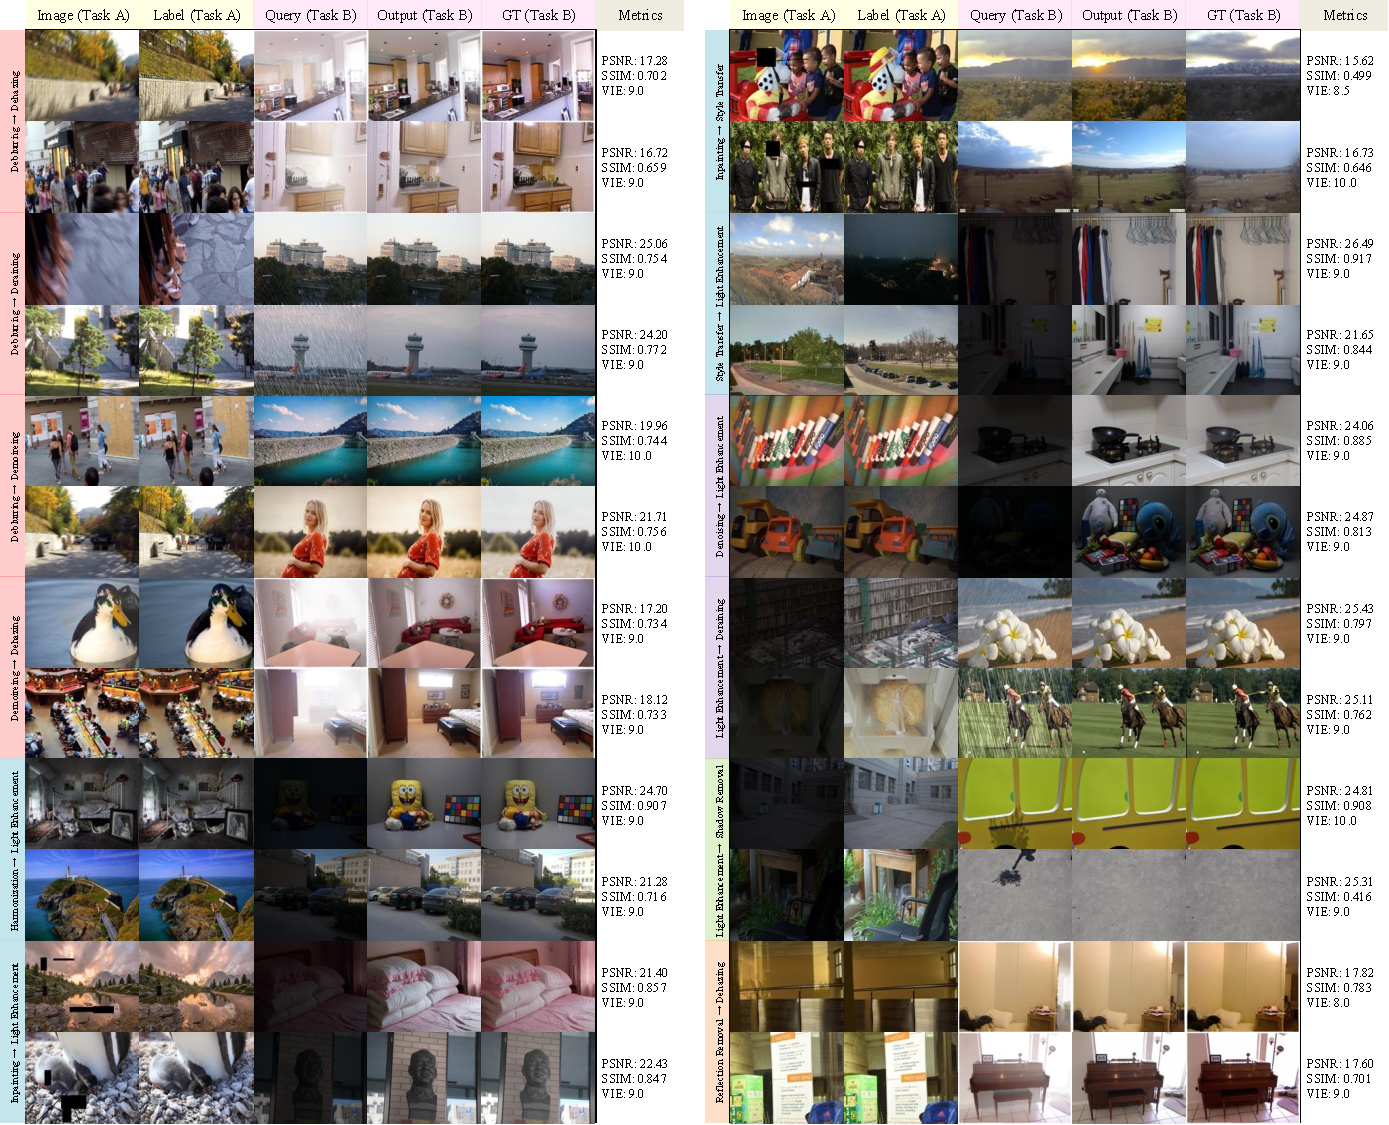
\includegraphics[width=\textwidth]{fig/figure4.pdf}
    \caption{Representative Examples of Cross-Task In-Context Learning from Gemini in Twelve Pairs}
    \label{fig:fig4}
\vspace{-8pt}
\end{figure*}

\subsection{Cross-Task Diversity and Adaptability}
The proposed VICL demonstrates consistent gains across diverse low-level vision tasks such as dehazing, deraining, demoireing. Beyond, the same prompting mechanism seamlessly extends to generation-oriented tasks such as low-light enhancement, effectively maintaining spatial layout and identity fidelity. Unlike prior approaches that are often confined to semantically similar domains, our method adapts seamlessly across both intra-category tasks (e.g., harmonization vs. light enhancement, demoireing vs. dehazing) and inter-category tasks (e.g., reflection removal vs. dehazing). These findings highlight the scalability and flexibility of our approach, showing that T2T-VICL can naturally bridge both perceptually related and unrelated tasks under a single model.

\subsection{Generalization to Distant Tasks} Beyond absolute numbers, an important property is cross-task consistency. This consistency underlines the advantage of framing all tasks under a unified in-context prompting mechanism. Moreover, T2T-VICL generalizes to semantically distant task pairs such as denoising versus light enhancement, where task-specialized models tend to degrade without task-specific retraining. This highlights robustness as a key byproduct of the unified in-context paradigm.

% \begin{table*}[ht]
% \centering
% \captionsetup{width=0.78\textwidth, skip=4pt, type=table}
% \caption{Average of evaluation metrics in the second-tier group. Generated by Gemini with Qwen prompts, compared to the fixed-prompt baseline.}
% \vspace{-1pt}

% \small
% % \scriptsize
% % \setlength{\tabcolsep}{4pt}
% % \renewcommand{\arraystretch}{1.0}

% \begin{tabularx}{0.785\textwidth}{lcccccc}
% \toprule
% \multirow{2}{*}{\textbf{Task}} & \multicolumn{2}{c}{\textbf{PSNR}$\uparrow$} & \multicolumn{2}{c}{\textbf{SSIM}$\uparrow$} & \multicolumn{2}{c}{\textbf{VIEScore}$\uparrow$} \\
%  & \textcolor{gray}{\textbf{Fixed}} & \textcolor{gray}{\textbf{Ours}}
%  & \textcolor{gray}{\textbf{Fixed}} & \textcolor{gray}{\textbf{Ours}}
%  & \textcolor{gray}{\textbf{Fixed}} & \textcolor{gray}{\textbf{Ours}} \\
% \midrule

% \rowcolor{lightred!30}
% Dehazing $\rightarrow$ Deraining             & \cellcolor{lightred!60}19.09 & 19.01 & \cellcolor{lightred!60}0.518 & 0.505 & 6.39 & \cellcolor{lightred!60}7.13 \\
% \rowcolor{lightred!30}
% Deraining $\rightarrow$ Demoireing             & \cellcolor{lightred!60}15.29 & 15.00 & \cellcolor{lightred!60}0.583 & 0.580 & 5.83 & \cellcolor{lightred!60}7.24 \\
% \rowcolor{lightblue!30}
% Colorization $\rightarrow$ Style Transfer    & \cellcolor{lightblue!60}13.35 & 13.03 & \cellcolor{lightblue!60}0.465 & 0.434 & 5.10 & \cellcolor{lightblue!60}7.37 \\
% \rowcolor{lightblue!30}
% Harmonization $\rightarrow$ Style Transfer   & \cellcolor{lightblue!60}13.32 & 13.14 & \cellcolor{lightblue!60}0.465 & 0.458 & 4.79 & \cellcolor{lightblue!60}5.66 \\
% \rowcolor{lightblue!30}
% Inpainting $\rightarrow$ Colorization        & \cellcolor{lightblue!60}21.31 & 20.75 & \cellcolor{lightblue!60}0.843 & 0.742 & 5.23 & \cellcolor{lightblue!60}7.39 \\
% \rowcolor{lightblue!30}
% Light Enhancement $\rightarrow$ Colorization & \cellcolor{lightblue!60}22.72 & 21.04 & \cellcolor{lightblue!60}0.860 & 0.753 & 5.05 & \cellcolor{lightblue!60}6.86 \\
% \rowcolor{lightpurple!30}
% Deraining $\rightarrow$ Style Transfer       & \cellcolor{lightpurple!60}13.31 & 13.10 & 0.430 & \cellcolor{lightpurple!60}0.447 & 4.67 & \cellcolor{lightpurple!60}5.66 \\
% \rowcolor{lightorange!30}
% Shadow Removal $\rightarrow$ Deraining       & \cellcolor{lightorange!50}19.49 & 18.98 & \cellcolor{lightorange!50}0.555 & 0.538 & 7.54 & \cellcolor{lightorange!50}8.20 \\
% \rowcolor{lightyellow!30}
% Shadow Removal $\rightarrow$ Reflection Removal & \cellcolor{lightyellow!50}21.79 & 21.44 & \cellcolor{lightyellow!50}0.761 & 0.739 & 6.24 & \cellcolor{lightyellow!50}6.34 \\
% \bottomrule
% \end{tabularx}
% \end{table*}



\begin{table*}[ht]
\centering
\scriptsize
\setlength{\tabcolsep}{0.5pt}
\renewcommand{\arraystretch}{0.96}
\captionsetup{width=0.98\textwidth, skip=4pt, type=table}
\caption{Average of evaluation metrics in the second-tier group. Generated by Gemini and Seedream with Qwen prompts, compared to the fixed-prompt baseline.}
% These task pairs consistently improve VIEScore for both Gemini and Seedream, while PSNR or SSIM may decrease.
\vspace{-1pt}
\label{tab:4}

\begin{adjustbox}{width=\textwidth}
\begin{tabular}{H *{5}{>{\centering\arraybackslash}m{0.8cm}} >{\centering\arraybackslash}m{1cm} *{5}{>{\centering\arraybackslash}m{0.8cm}} >{\centering\arraybackslash}m{1cm}}
\toprule
\multirow{3}{*}{\textbf{Task}}
& \multicolumn{6}{c}{\textbf{Gemini 2.5 Flash}}
& \multicolumn{6}{c}{\textbf{Seedream 4.0}} \\
& \multicolumn{2}{c}{\textbf{PSNR}$\uparrow$}
& \multicolumn{2}{c}{\textbf{SSIM}$\uparrow$}
& \multicolumn{2}{c}{\textbf{VIEScore}$\uparrow$}
& \multicolumn{2}{c}{\textbf{PSNR}$\uparrow$}
& \multicolumn{2}{c}{\textbf{SSIM}$\uparrow$}
& \multicolumn{2}{c}{\textbf{VIEScore}$\uparrow$} \\
& \textcolor{gray}{\textbf{Fixed}} & \textcolor{gray}{\textbf{Ours}}
& \textcolor{gray}{\textbf{Fixed}} & \textcolor{gray}{\textbf{Ours}}
& \textcolor{gray}{\textbf{Fixed}} & \textcolor{gray}{\textbf{Ours}}
& \textcolor{gray}{\textbf{Fixed}} & \textcolor{gray}{\textbf{Ours}}
& \textcolor{gray}{\textbf{Fixed}} & \textcolor{gray}{\textbf{Ours}}
& \textcolor{gray}{\textbf{Fixed}} & \textcolor{gray}{\textbf{Ours}} \\
\midrule

\rowcolor{lightred!30}
\makecell[l]{Dehazing $\rightarrow$ Deraining}
& \cellcolor{lightred!60}19.09 & 19.01
& \cellcolor{lightred!60}0.518 & 0.505
& 6.39 & \cellcolor{lightred!60}\tabgainsubscript{7.13}{+0.74}
& 14.47 & \cellcolor{lightred!60}14.49
& 0.385 & \cellcolor{lightred!60}0.386
& 6.41 & \cellcolor{lightred!60}\tabgainsubscript{6.76}{+0.35} \\
\grayhline

\rowcolor{lightred!30}
\makecell[l]{Deraining $\rightarrow$ Demoireing}
& \cellcolor{lightred!60}15.29 & 15.00
& \cellcolor{lightred!60}0.583 & 0.580
& 5.83 & \cellcolor{lightred!60}\tabgainsubscript{7.24}{+1.41}
& \cellcolor{lightred!60}11.84 & 10.95
& \cellcolor{lightred!60}0.451 & 0.418
& 7.38 & \cellcolor{lightred!60}\tabgainsubscript{7.40}{+0.02} \\
\grayhline

\rowcolor{lightblue!30}
\makecell[l]{Colorization $\rightarrow$ Style Transfer}
& \cellcolor{lightblue!60}13.35 & 13.03
& \cellcolor{lightblue!60}0.465 & 0.434
& 5.10 & \cellcolor{lightblue!60}\tabgainsubscript{7.37}{+2.27}
& \cellcolor{lightblue!60}9.91 & 9.54
& \cellcolor{lightblue!60}0.333 & 0.314
& 7.99 & \cellcolor{lightblue!60}\tabgainsubscript{8.09}{+0.10} \\
\grayhline

\rowcolor{lightblue!30}
\makecell[l]{Harmonization $\rightarrow$ Style Transfer}
& \cellcolor{lightblue!60}13.32 & 13.14
& \cellcolor{lightblue!60}0.465 & 0.458
& 4.79 & \cellcolor{lightblue!60}\tabgainsubscript{5.66}{+0.87}
& \cellcolor{lightblue!60}10.20 & 9.63
& \cellcolor{lightblue!60}0.354 & 0.331
& 7.32 & \cellcolor{lightblue!60}\tabgainsubscript{7.62}{+0.30} \\
\grayhline

\rowcolor{lightblue!30}
\makecell[l]{Inpainting $\rightarrow$ Colorization}
& \cellcolor{lightblue!60}21.31 & 20.75
& \cellcolor{lightblue!60}0.843 & 0.742
& 5.23 & \cellcolor{lightblue!60}\tabgainsubscript{7.39}{+2.16}
& \cellcolor{lightblue!60}13.53 & 12.08
& \cellcolor{lightblue!60}0.447 & 0.397
& 5.86 & \cellcolor{lightblue!60}\tabgainsubscript{6.96}{+1.10} \\
\grayhline

\rowcolor{lightblue!30}
\makecell[l]{Light Enhancement $\rightarrow$ Colorization}
& \cellcolor{lightblue!60}22.72 & 21.04
& \cellcolor{lightblue!60}0.860 & 0.753
& 5.05 & \cellcolor{lightblue!60}\tabgainsubscript{6.86}{+1.81}
& 11.01 & \cellcolor{lightblue!60}12.09
& \cellcolor{lightblue!60}0.436 & 0.422
& 4.59 & \cellcolor{lightblue!60}\tabgainsubscript{7.28}{+2.69} \\
\grayhline

\rowcolor{lightyellow!30}
\makecell[l]{Shadow Removal $\rightarrow$ Reflection Removal}
& \cellcolor{lightyellow!50}21.79 & 21.44
& \cellcolor{lightyellow!50}0.761 & 0.739
& 6.24 & \cellcolor{lightyellow!50}\tabgainsubscript{6.34}{+0.10}
& \cellcolor{lightyellow!50}14.96 & 13.10
& \cellcolor{lightyellow!50}0.532 & 0.459
& 7.13 & \cellcolor{lightyellow!50}\tabgainsubscript{7.17}{+0.04} \\
\grayhline

\rowcolor{lightpurple!30}
\makecell[l]{Deraining $\rightarrow$ Style Transfer}
& \cellcolor{lightpurple!60}13.31 & 13.10
& 0.430 & \cellcolor{lightpurple!60}0.447
& 4.67 & \cellcolor{lightpurple!60}\tabgainsubscript{5.66}{+0.99}
& \cellcolor{lightpurple!60}11.02 & 9.76
& \cellcolor{lightpurple!60}0.375 & 0.318
& 6.66 & \cellcolor{lightpurple!60}\tabgainsubscript{7.33}{+0.67} \\
\grayhline

\rowcolor{lightorange!30}
\makecell[l]{Shadow Removal $\rightarrow$ Deraining}
& \cellcolor{lightorange!50}19.49 & 18.98
& \cellcolor{lightorange!50}0.555 & 0.538
& 7.54 & \cellcolor{lightorange!50}\tabgainsubscript{8.20}{+0.66}
& \cellcolor{lightorange!50}17.37 & 15.25
& \cellcolor{lightorange!50}0.487 & 0.431
& 7.51 & \cellcolor{lightorange!50}\tabgainsubscript{7.68}{+0.17} \\
\bottomrule
\end{tabular}
\end{adjustbox}
\vspace{-6pt}
\end{table*}


\subsection{Cross-Task Results in Second-Tier Group}
Across another nine cross-task pairs in Table~\ref{tab:4}, our method consistently improves VIEScore over the fixed-prompt baseline on both Gemini and Seedream. The other two IQA metrics have slight declines in several cases. Interestingly, for these compositions, improvements are primarily reflected in the VIEScore rather than in the traditional fidelity metrics. Since VIE measures structural and relational coherence of visual information, it is more sensitive to semantic preservation than to strict intensity alignment. See detailed discussion in Appendix Sec.~\ref{sec:viescore}.

% \vspace{1pt}
% \noindent
% \begin{minipage}{\columnwidth}
% \centering
% \captionsetup{font=scriptsize, width=\columnwidth, skip=1pt}
% \captionof{table}{Avg of metrics for ablation study on effects of prompt enhancement and ICL.}
% % (1) One input image + training data copied long fixed prompt;
% % (2) Image 1-3 all from same task, clear fixed prompt (same task);
% % (3) Image 1-3 all from same task, long prompt (image descriptions + visual changes).
% \label{tab:r2}
% \scriptsize
% \setlength{\tabcolsep}{1.48pt}
% \renewcommand{\arraystretch}{0.927}
% \begin{tabularx}{\columnwidth}{S*{9}{C}}
% \toprule
% \multirow{2}{*}{\textbf{Task}} 
% & \multicolumn{3}{c}{\textbf{Prompt-only}} 
% & \multicolumn{3}{c}{\textbf{Same-task ICL+Fix}} 
% & \multicolumn{3}{c}{\textbf{Same-task ICL+Enh}} \\
% & PSNR & SSIM & VIE
% & PSNR & SSIM & VIE
% & PSNR & SSIM & VIE \\
% \midrule

% \rowcolor{lightred!30}
% Deblurring
% & 20.14 & 0.597 & 4.66
% & 17.51 & 0.529 & \cellcolor{lightred!60}4.69
% & \cellcolor{lightred!60}19.29 & \cellcolor{lightred!60}0.578 & 4.30 \\

% \rowcolor{lightred!30}
% Dehazing
% & 13.08 & 0.541 & 8.05
% & 12.47 & 0.510 & 6.78
% & \cellcolor{lightred!60}12.68 & \cellcolor{lightred!60}0.511 & \cellcolor{lightred!60}6.92 \\

% \rowcolor{lightred!30}
% Demoireing
% & 15.88 & 0.588 & 8.87
% & 14.98 & 0.574 & 7.41
% & \cellcolor{lightred!60}15.89 & \cellcolor{lightred!60}0.596 & \cellcolor{lightred!60}7.57 \\

% \rowcolor{lightred!30}
% Deraining
% & 20.40 & 0.591 & 8.62
% & 19.61 & 0.563 & 7.31
% & \cellcolor{lightred!60}19.86 & \cellcolor{lightred!60}0.575 & \cellcolor{lightred!60}8.00 \\

% \rowcolor{lightblue!30}
% Colorization
% & 20.61 & 0.722 & 8.69
% & \cellcolor{lightblue!60}21.18 & \cellcolor{lightblue!60}0.788 & 6.51
% & 20.68 & 0.755 & \cellcolor{lightblue!60}7.29 \\

% \rowcolor{lightblue!30}
% Harmonization
% & 19.71 & 0.592 & 9.77
% & 19.88 & 0.648 & \cellcolor{lightblue!60}6.65
% & \cellcolor{lightblue!60}20.18 & \cellcolor{lightblue!60}0.662 & 6.61 \\

% \rowcolor{lightblue!30}
% Inpainting
% & 18.81 & 0.516 & 9.12
% & 18.18 & 0.544 & 8.31
% & \cellcolor{lightblue!60}18.81 & \cellcolor{lightblue!60}0.547 & \cellcolor{lightblue!60}8.65 \\

% \rowcolor{lightblue!30}
% Light Enh.
% & 14.37 & 0.576 & 8.98
% & 12.27 & 0.482 & 8.26
% & \cellcolor{lightblue!60}14.00 & \cellcolor{lightblue!60}0.574 & \cellcolor{lightblue!60}8.92 \\

% \rowcolor{lightblue!30}
% Style Trans.
% & 13.24 & 0.444 & 8.58
% & 12.96 & \cellcolor{lightblue!60}0.452 & \cellcolor{lightblue!60}6.69
% & \cellcolor{lightblue!60}13.08 & 0.446 & 6.42 \\

% \rowcolor{lightyellow!30}
% Refl. Rmv.
% & 22.19 & 0.753 & 7.78
% & 20.13 & 0.718 & 5.84
% & \cellcolor{lightyellow!60}22.25 & \cellcolor{lightyellow!60}0.766 & \cellcolor{lightyellow!60}5.90 \\

% \rowcolor{lightyellow!30}
% Shadow Rmv.
% & 19.19 & 0.338 & 8.87
% & \cellcolor{lightyellow!60}18.72 & \cellcolor{lightyellow!60}0.334 & 7.47
% & 18.58 & 0.333 & \cellcolor{lightyellow!60}8.31 \\

% \bottomrule
% \end{tabularx}
% \end{minipage}
% \vspace{-4pt}


\vspace{6pt}
\noindent
\begin{minipage}{\columnwidth}
\centering
\captionsetup{width=0.99\columnwidth, skip=4pt, type=table}
\captionof{table}{Average of metrics for ablation study on effects of prompt enhancement and ICL, generated by Gemini.}
% (1) One input image + training data copied long fixed prompt;
% (2) Image 1-3 all from same task, clear fixed prompt (same task);
% (3) Image 1-3 all from same task, long prompt (image descriptions + visual changes).
\label{tab:6}
\scriptsize
\setlength{\tabcolsep}{2pt}
\renewcommand{\arraystretch}{0.95}
\begin{tabularx}{\columnwidth}{l*{6}{C}}
\toprule
\multirow{2}{*}{\textbf{Task}} 
% & \multicolumn{3}{c}{\textbf{Prompt-only}} 
& \multicolumn{3}{c}{\textbf{Same-task ICL + Fixed}} 
& \multicolumn{3}{c}{\textbf{Same-task ICL + Enh.}} \\
% & PSNR & SSIM & VIE
& PSNR & SSIM & VIE
& PSNR & SSIM & VIE \\
\midrule

\rowcolor{lightred!30}
Deblurring
% & 20.14 & 0.597 & 4.66
& 17.51 & 0.529 & \cellcolor{lightred!60}4.69
& \cellcolor{lightred!60}19.29 & \cellcolor{lightred!60}0.578 & 4.30 \\

\rowcolor{lightred!30}
Dehazing
% & 13.08 & 0.541 & 8.05
& 12.47 & 0.510 & 6.78
& \cellcolor{lightred!60}12.68 & \cellcolor{lightred!60}0.511 & \cellcolor{lightred!60}6.92 \\

\rowcolor{lightred!30}
Demoireing
% & 15.88 & 0.588 & 8.87
& 14.98 & 0.574 & 7.41
& \cellcolor{lightred!60}15.89 & \cellcolor{lightred!60}0.596 & \cellcolor{lightred!60}7.57 \\

\rowcolor{lightred!30}
Deraining
% & 20.40 & 0.591 & 8.62
& 19.61 & 0.563 & 7.31
& \cellcolor{lightred!60}19.86 & \cellcolor{lightred!60}0.575 & \cellcolor{lightred!60}8.00 \\

\rowcolor{lightblue!30}
Colorization
% & 20.61 & 0.722 & 8.69
& \cellcolor{lightblue!60}21.18 & \cellcolor{lightblue!60}0.788 & 6.51
& 20.68 & 0.755 & \cellcolor{lightblue!60}7.29 \\

\rowcolor{lightblue!30}
Harmonization
% & 19.71 & 0.592 & 9.77
& 19.88 & 0.648 & \cellcolor{lightblue!60}6.65
& \cellcolor{lightblue!60}20.18 & \cellcolor{lightblue!60}0.662 & 6.61 \\

\rowcolor{lightblue!30}
Inpainting
% & 18.81 & 0.516 & 9.12
& 18.18 & 0.544 & 8.31
& \cellcolor{lightblue!60}18.81 & \cellcolor{lightblue!60}0.547 & \cellcolor{lightblue!60}8.65 \\

\rowcolor{lightblue!30}
Light Enhancement
% & 14.37 & 0.576 & 8.98
& 12.27 & 0.482 & 8.26
& \cellcolor{lightblue!60}14.00 & \cellcolor{lightblue!60}0.574 & \cellcolor{lightblue!60}8.92 \\

\rowcolor{lightblue!30}
Style Transfer
% & 13.24 & 0.444 & 8.58
& 12.96 & \cellcolor{lightblue!60}0.452 & \cellcolor{lightblue!60}6.69
& \cellcolor{lightblue!60}13.08 & 0.446 & 6.42 \\

\rowcolor{lightyellow!30}
Reflection Removal
% & 22.19 & 0.753 & 7.78
& 20.13 & 0.718 & 5.84
& \cellcolor{lightyellow!60}22.25 & \cellcolor{lightyellow!60}0.766 & \cellcolor{lightyellow!60}5.90 \\

\rowcolor{lightyellow!30}
Shadow Removal
% & 19.19 & 0.338 & 8.87
& \cellcolor{lightyellow!60}18.72 & \cellcolor{lightyellow!60}0.334 & 7.47
& 18.58 & 0.333 & \cellcolor{lightyellow!60}8.31 \\

\bottomrule
\end{tabularx}
% \vspace{3pt}
\end{minipage}


\subsection{Ablation Study}

We further investigate the scalability of our method under the traditional same-task VICL setting. Specifically, we conduct ablation studies on Gemini to validate the performance gains of T2T-VICL by: (1) applying VICL to the same task with a fixed prompt, and (2) applying VICL to the same task with an implicitly enriched prompt derived from same task samples using a similar pipeline as T2T-VICL. 
Details of the two prompt configurations are provided in Sec.~\ref{sec:prompt} in Appendix.
Table~\ref{tab:6} reports the results of same-task VICL with fixed and enhanced prompts.
Experimental results demonstrate improvements in PSNR, SSIM, and VIEScore across multiple task pairs.


\subsection{Discussion}
Overall, our framework demonstrates strong one-shot generalization and robust visual consistency across a wide range of low-level vision tasks. By leveraging implicit prompt representations, the model effectively adapts to unseen task combinations without task-specific fine-tuning, achieving top-tier VIEScores in many cases. However, due to the inherent complexity of cross-task compositions, a few cases with limited reference samples occasionally produce content that does not exist in the original images, slightly lowering the fidelity-based indicators. Despite these imperfections, the overall visual consistency remains close to that of the top group. Future work will focus on adaptive balancing between semantic-level and pixel-level objectives to further improve realism and generalization across diverse unseen conditions.
